\section{Experimental Setup}
\label{sec:setup}
\paragraph{Controlled payment boundaries.}
We construct 200 tasks from 20 contract templates in four families: coupon cancellation, insured cancellation, threshold-dependent returns, and service replacement. Contracts combine overlapping groups, compensation layers, shipping charges, and item/order caps. Each purchase has six components. The event universe contains all affected subsets of size at most four, including the empty event: 57 states per candidate. Catalogues contain 128--1,024 candidates. All amounts use abstract monetary units (MU), with 100 integer subunits per MU. Exact arithmetic on subunits preserves strict and inclusive financial boundaries.



Each template contributes five feasible/infeasible pairs. A feasible task has exactly one authorized positive-value candidate. A fee perturbation determined by its feasible margin moves its worst loss exactly one subunit above the limit; other attributes and offer order stay fixed. These 100 pairs isolate responsiveness to authorization boundaries \citep{checklist,contrastsets,hans}, rather than estimating deployment error rates or broad ranking ability. Separate cash-ledger and expression implementations agree on 6,712,320 candidate--event checks, supplemented by 25,600 random-attribute checks and three hand-calculated witnesses. This checks consistency with stipulated synthetic semantics; both implementations arose within one development workflow. Inputs and references were frozen before primary calls (Appendix~\ref{app:data}).

\begin{figure*}[t]
\centering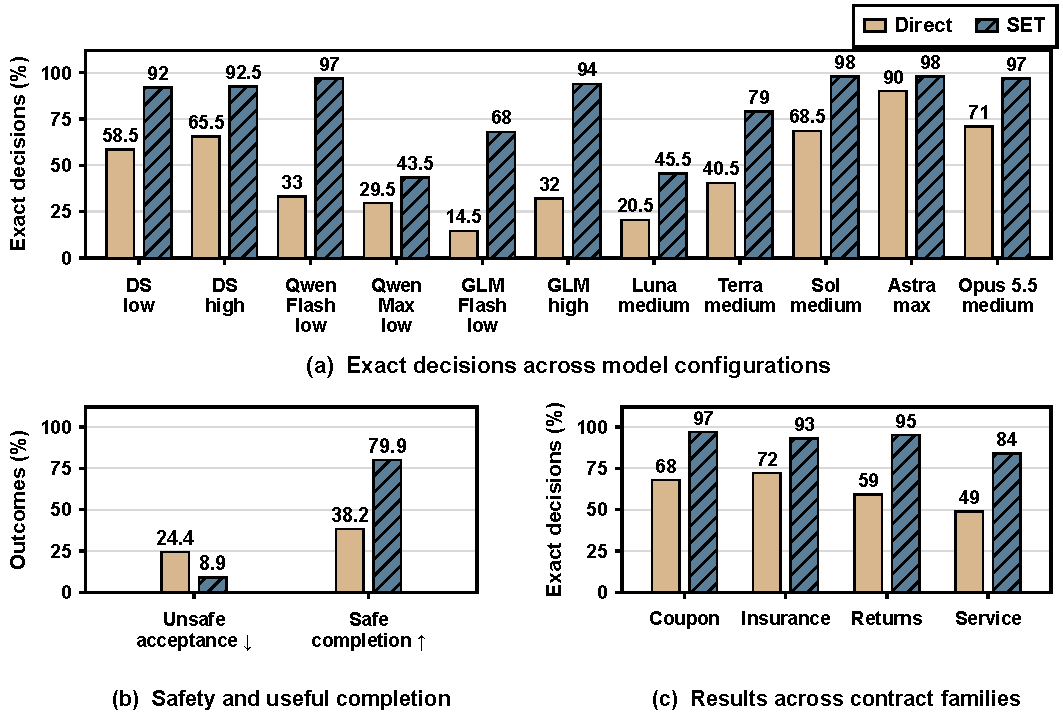
\includegraphics[width=\textwidth]{14_safe_completion.pdf}
\caption{\textbf{Risk-aware decisions across models and contract structures.} Each group compares Direct and Set. (a) Exact-decision rates across model configurations. (b) All eleven configurations: unsafe acceptance over 2,200 task--configuration outcomes and safe completion over 1,100 feasible outcomes per method. (c) DeepSeek low/high across four contract families, each pooling 100 outcomes from five templates. All axes start at zero; failures remain in the denominators. Configurations share task sets.}
\label{fig:completion}
\end{figure*}

\paragraph{Comparisons.}
The \direct--\ours\ comparison evaluates the complete executable decision architecture under a shared decision policy. \direct\ receives the request, schema, full catalogue, and robust decision rules; it returns a decision, selected identifiers, and guaranteed utility. \ours\ compiles a catalogue-independent rule for the fixed evaluator. Appendix~\ref{app:execution} adds a generic prompt engineering checklist and Set-Py, a procedural realization of the same framework. Both executable realizations improve over Direct and the tested checklist in the matched panel; their relative reliability varies by configuration. These controls support executable processing, not universal superiority of one encoding.

The primary comparison spans eleven model configurations: Astra max; Sol, Terra, and Luna medium; DeepSeek low and high; Qwen Flash and Max low; GLM Flash low and GLM high; and Opus 5.5 medium. Cohort definitions are in Appendix~\ref{app:primary-extensions}; other panels retain their own cohorts.

\paragraph{Outcome scoring.}
An \emph{exact decision} agrees with the reference decision and, for acceptance, reports authorized maximizing choices and correct utility. \emph{Safe task completion} is exact acceptance on a feasible task. \emph{Unsafe acceptance} returns a reference-infeasible choice; \emph{false refusal} rejects an available positive-value authorized purchase. Other groups remaining value and invalid-execution failures; all failures stay in the denominator. Archived outcome agreement and full-domain certification are distinguished in Appendix~\ref{app:interface}. Authorization auditing also checks unselected admitted candidates. Trials retain one semantic attempt, bounded transport retries, responses, usage, duration, and evaluation. Syntax recovery preserves expression meaning. Comparisons are paired within configurations; provider compute budgets are not equivalent.

\paragraph{Reproducibility.}
The anonymous artifact provides code, benchmark inputs and references, prompts, configurations, retained responses, and evaluation records. An offline entry reconstructs tables and figures, checks paired outcome partitions and Algorithm~\ref{alg:decision}, and records input hashes without model calls. Appendix~\ref{app:reproduction} maps results to records and verification tools; Table~\ref{tab:configurations} specifies generation settings.

\section{Results and Analysis}
\label{sec:evaluation}
\label{sec:results}
Table~\ref{tab:evaluation-coverage} connects four questions: useful completion at risk boundaries, decisions across retained readings, the semantics concealed by current choices, and robustness and reuse. Each study retains its own input conditions and sample unit.

\subsection{Safe Completion under Contractual Uncertainty}
\label{sec:boundaries}



Figure~\ref{fig:completion} combines model coverage, joint safety--completion outcomes, and contract-level variation. All eleven configurations improve exactness, reduce unsafe acceptances, and complete more authorized purchases. Across the two primary DeepSeek configurations, exact decisions rise from 248/400 (62.0\%) to 370/400 (92.5\%). The gain is 30.5 percentage points, with a 95\% template-cluster bootstrap interval of $[22.75,37.75]$, retaining both settings within each template. Exact purchases rise from 100 to 186 across 200 feasible outcomes, while unsafe acceptances fall from 79 to 9 and false refusals from 53 to 1. Safety improves together with useful completion.

Each pair changes one fee and requires opposite decisions, testing more than blanket acceptance or refusal. The gains concern the full compilation-and-execution workflow; this comparison does not isolate catalogue visibility, exact arithmetic, state representation, and deterministic evaluation.

The updated Astra max comparison scores 180/200 (90\%) for direct answering and 196/200 (98\%) for \ours. Direct has six unsafe acceptances, six false refusals, and eight Other failures; \ours\ has two unsafe acceptances and two false refusals. Traced errors from the original archived run illustrate both boundary failures (Appendix~\ref{app:witnesses}).

\subsection{Decisions under Signaled Intent Ambiguity}
\label{sec:intent-decisions}
Figure~\ref{fig:intent} reports 294 method outcomes from 147 matched task--configuration units across three intent families: ticket-holder reference, conditional hotel cancellation, and per-recipient versus whole-batch exchange-cost limits. Both methods receive the same catalogue, explicit ambiguity cues, and decision rules, without further user input. Unlike the primary Set protocol, compilation here is catalogue-visible. Table~\ref{tab:intent-figure3} gives configuration-specific denominators; Appendix~\ref{app:intent} relates them to the broader archive.

\begin{figure}[t]
\centering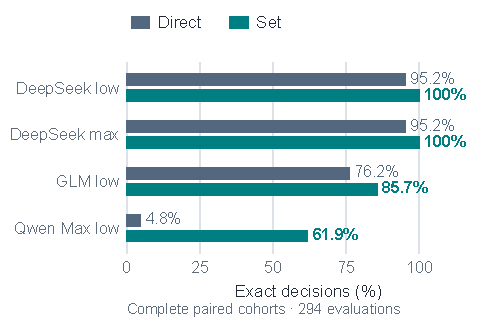
\includegraphics[width=\columnwidth]{16_retained_intent.pdf}
\caption{\textbf{Decisions with unresolved user intent.} Exact-decision rates in complete paired API cohorts. Percentages use each configuration's own denominator, retaining failures. Counts, error categories, and the full study are in Appendix~\ref{app:intent}.}
\label{fig:intent}
\end{figure}

Exactness improves across the four configurations as risk limits, penalties, and the positive-value boundary vary. Safety does not improve uniformly: Qwen has six unsafe Set acceptances versus five for Direct. The capability checks illustrated by Table~\ref{tab:observed-trace} additionally exercise common purchases, empty intersections, and max--min ranking. All compared routes solve those small checks; they establish behavior coverage, not a comparative ranking advantage.

\subsection{Correct Choices Can Conceal Unsafe Authorization}
\label{sec:permissions}
\label{sec:components}
\paragraph{Candidate changes expose hidden permissions.}
We freeze 648 DeepSeek artifacts from 72 tasks, three effort settings, and three realizations: Set, catalogue-visible Set-Py, and matched-input Set-Py. Across 1,296 local replays, valid mixed-catalogue executions select no unauthorized offer, although 23 artifacts admit one. Eight select an unauthorized offer when the catalogue contains only that option (Figure~\ref{fig:ablations}); 12 artifacts have invalid executions per condition. No model is called again. Changing availability exposes an error that the original safe selection concealed, rather than measuring a deployment failure rate (Appendix~\ref{app:permissionaudit}).

\begin{figure}[t]
\centering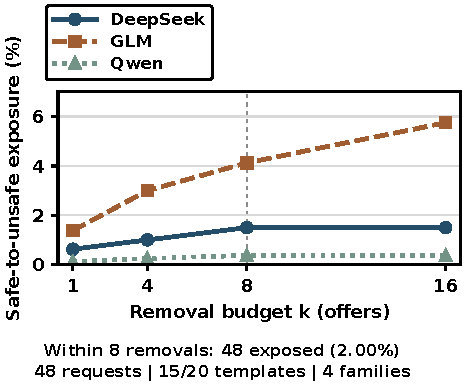
\includegraphics[width=\columnwidth]{13_authorization_diagnostics.pdf}
\caption{\textbf{A safe choice can mask an unsafe rule.} Frozen DeepSeek artifacts admit unauthorized candidates in mixed catalogues; some select them in unsafe-only catalogues. Valid mixed-catalogue runs make no unsafe selections. Each configuration pools 216 artifacts across three realizations; invalid executions are counted separately.}
\label{fig:ablations}
\end{figure}

\paragraph{Correcting value alone can expose a permission error.}
Table~\ref{tab:oracle} intervenes on 16 faulty Set outputs selected from one ambiguous ticket request. All omit Li's refund conditions and utility binding. Their current selections are safe despite incorrect domains and values. Replacing only utility with the reference makes an unauthorized offer win in all 16 outputs. Replacing permission alone repairs the domain but not value; replacing both, or restoring the omitted state's complete semantics, recovers exact decisions. Thus ranking errors can temporarily mask authorization errors. The interventions identify a failure mechanism, not its prevalence or an automatic repair procedure.

\begin{table}[t]
\centering\small\setlength{\tabcolsep}{4pt}
\begin{tabular}{@{}lrrr@{}}
\toprule
Intervention & Exact & Unsafe & Unsafe domain\\
\midrule
Original & 0 & 0 & 16\\
Duplicate label & 0 & 0 & 16\\
Reference permission & 0 & 0 & 0\\
Reference utility & 0 & 16 & 16\\
Both components & 16 & 0 & 0\\
Restore omitted state & 16 & 0 & 0\\
\bottomrule
\end{tabular}
\caption{\textbf{Permission and value are distinct checks.} Counts are out of 16 selected faulty outputs, not independent requests. Unsafe counts selections; Unsafe domain counts rules admitting an unauthorized candidate. Interventions use reference information offline (Appendix~\ref{app:oracle}).}
\label{tab:oracle}
\end{table}

\paragraph{Why retained states matter.}
For fixed $x$ and unchanged remaining state functions, retaining only $\varnothing\ne\Theta'\subseteq\Theta$ gives
\[
F_{\Theta}\subseteq F_{\Theta'},\qquad
\psi_{\Theta'}(z)\ge\psi_{\Theta}(z).
\]
Fewer conjuncts cannot shrink feasibility, and fewer terms cannot lower an infimum. This consequence of Equations~\eqref{eq:common}--\eqref{eq:robust} explains why a missing reading can enlarge permission and inflate guaranteed value simultaneously. It concerns semantic deletion, not an equivalent merging of states. Together, the replays and interventions motivate checking authorization and value separately from the current action.

\subsection{Robustness across Structures and Settings}
\label{sec:robustness}
Improvements cover all four financial families (Figure~\ref{fig:completion}c) and 18 of 20 templates at each DeepSeek setting. Across models, GLM high improves from 64/200 to 188/200, Sol medium from 137/200 to 196/200, and Opus medium from 142/200 to 194/200. The gains vary: Qwen Max low increases from 59 to 87 exact outcomes while retaining 46 unsafe acceptances. Full partitions and template results are in Appendix~\ref{app:statistics}.

On the 60-task effort panel, \ours\ improves exactness in 18 of 19 complete GPT-5.6 configurations, including Sol ultra; Luna with reasoning disabled declines from 25/60 to 14/60. Figure~\ref{fig:robustness} and Table~\ref{tab:grid} report all 19 settings. Matched task-language tests preserve identifiers, quantities, events, and authorization; the DeepSeek improvements persist in both Chinese and English. These checks retain semantic and operational failures. Full effort, language, and budget controls are in Appendix~\ref{app:execution}.

\subsection{Reuse and Execution Cost}
\label{sec:reuse}
Across two fixed requirements and eight catalogue snapshots each, Astra uses two Set compilations and 22,160 tokens instead of 16 Direct calls and 175,429 tokens, with 16/16 exact decisions in both workflows (Table~\ref{tab:reuse-main}). This 87.4\% workflow-level token reduction includes initial compilation; it does not isolate caching within a single implementation. Reuse requires stable authorization; changed requirements trigger recompilation. Appendix~\ref{app:cost} gives full resource accounting.

\begin{table}[t]
\centering\small
\begin{tabular}{@{}lrrr@{}}
\toprule
Astra workflow & Calls & Tokens & Exact\\
\midrule
Direct per catalogue & 16 & 175,429 & 16/16\\
Set with rule reuse & 2 & 22,160 & 16/16\\
\bottomrule
\end{tabular}
\caption{\textbf{Reuse includes the first compilation.} Two fixed requirements, eight catalogues each; tokens include recorded input and output usage.}
\label{tab:reuse-main}
\end{table}
